\appendix
%\chapter*{Annexes}
\thispagestyle{empty}
\addcontentsline{toc}{chapter}{Annexes}
\renewcommand{\chaptermark}{Annexes}
\renewcommand\thesection{A\arabic{section}}

	\clearpage
	\section{Abaques de vapeur}

		\begin{center}
	Les données suivantes présentent les propriétés de l’eau pure sur une large plage de propriétés.\\
	Elles sont calculées à partir du modèle NIST-IAPWS 1995.

	L’énergie interne spécifique $u$ et l’entropie spécifique $s$ \\
	sont arbitrairement posées comme nulles au point triple de l’eau.

	Licence: Mise en page \cczero (Olivier Cleynen) ; données \pd (USA NIST).
	%Un ensemble d’abaques plus complet est téléchargeable à l’adresse \href{http://abaques.ariadacapo.net/}{http://abaques.ariadacapo.net/}.
\end{center}


	\clearpage
	\newgeometry{top=1cm, bottom=1cm, left=1cm, right=1cm}
	\begin{spacing}{1.06}
	\pagestyle{empty}
	\titleformat{\subsection}{\normalsize\center}{\thesection.}{0.5em}{}[\vspace{-0.5cm}]
		%%%%%%%%%%%%%%%%%%%%%%%%%%%%%%%%%%%%%%%%%%%%
		% LEZABAK LEZABAK
			%% Ce document simule la compilation des 8 pages d’abaques de vapeur,
% qui prend plusieurs minutes, pour permettre une compilation temporaire plus rapide.

\vspace*{\stretch{1}}
\begin{center}
	Ici, 8 pages A4, ommises pour réduire le temps de compilation :
	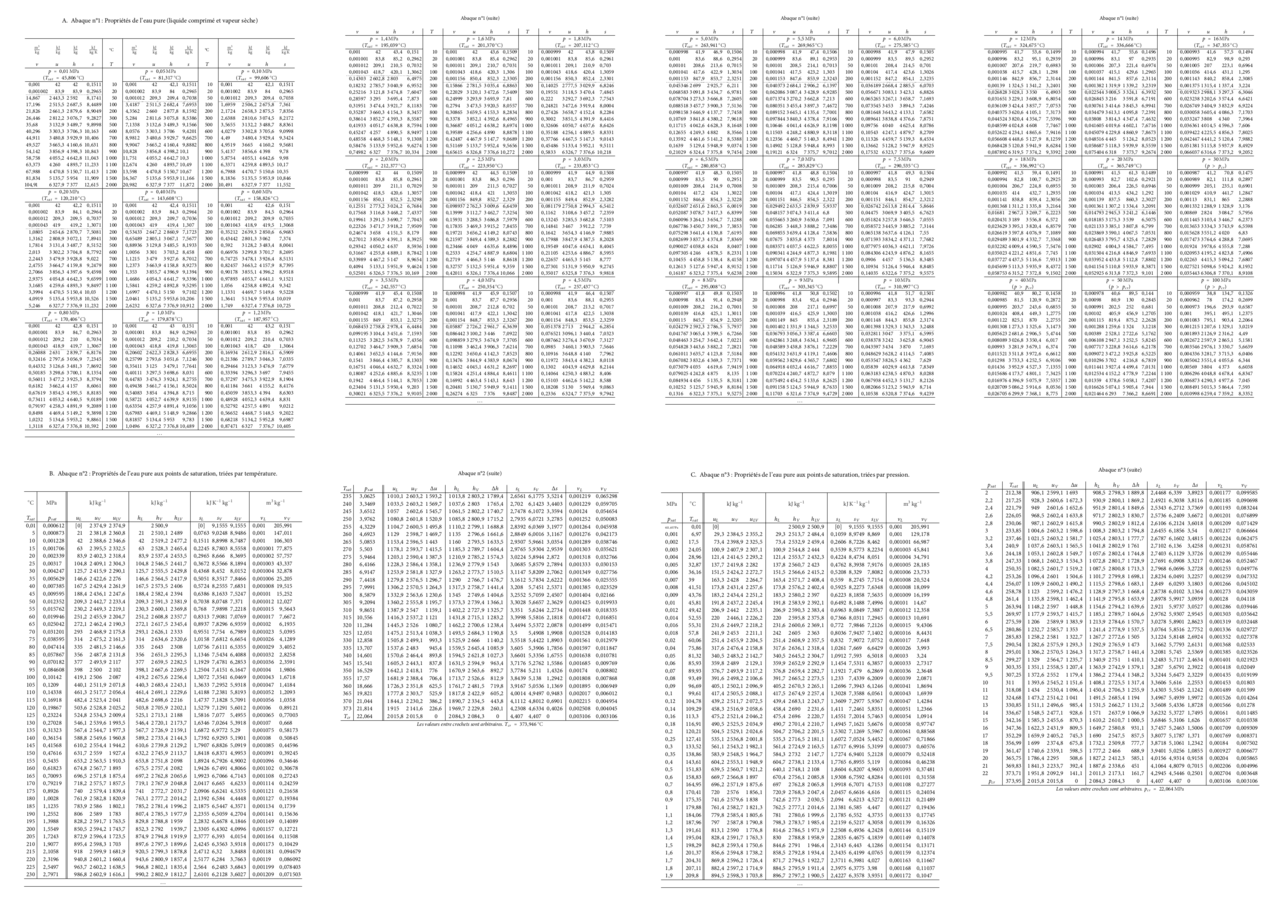
\includegraphics[width=\textwidth]{images/abaques.png}
	Elles sont consultables séparément dans le fichier \url{framabok/annexes/abaques_vapeur.pdf}
\end{center}
\vspace*{\stretch{1}}
 % activer cette ligne et commenter celle du dessous pour accélérer la compilation du livre
			../../contenu/Annexes/contenu_abaques_vapeur.tex
		% LEZABAK LEZABAK
		%%%%%%%%%%%%%%%%%%%%%%%%%%%%%%%%%%%%%%%%%%%%
	\clearpage\pagestyle{fancy}
	\end{spacing}%
	\restoregeometry%


	\section[Pression indiquée et pression réelle]{Distinction entre pression indiquée et pression réelle}
	\label{ch_annexe_pression}

				
		La pression indiquée sur un baromètre n’est pas toujours la pression réelle du fluide.
		
		En effet, on mesure souvent la pression à l’aide de manomètres qui sont calibrés sur la pression atmosphérique. Par exemple, lorsque l’on regonfle un pneu en station-service, le manomètre indique \SI{0}{\bar} à pression ambiante --\ toutes les pressions qu’il indiquera seront décalées de la valeur de la pression atmosphérique. Nous nommons cette valeur indiquée la \textbf{\vocab{pression jaugée}}.

		La pression jaugée se définit comme :
		\begin{equation*}
		p_{\text{j}} \equiv  p_{\text{réelle}} - p_{\text{atm.}}
		\end{equation*}
		
		\begin{equationterms}
			\item où \tab $p_{\text{j}}$ 			\tab\tab est la pression jaugée, indiquée au cadran (\si{\pascal}),
			\item 	\tab $p_{\text{réelle}}$	\tab est la pression réelle au sein du réservoir où est faite la mesure (\si{\pascal}),
			\item et \tab $p_{\text{atm.}}$ 		\tab\tab est la pression atmosphérique ambiante (\si{\pascal}).
		\end{equationterms}

		Un manomètre jaugé indique donc \SI{0}{\bar} quelle que soit la pression ambiante, s’il est laissé à l’air libre. La pression indiquée lors d’une mesure dépendra de la pression atmosphérique ambiante ; elle peut être positive (pneu) ou parfois négative (conduit d’eau ou de pétrole).
		
		La pression jaugée est intéressante parce qu’elle indique \emph{la différence} de pression entre chacun des côtés des parois du réservoir (pneu, canalisation) ; elle révèle donc les contraintes qu’elles subissent. La pression réelle de l’air à l’intérieur du pneu n’a pas d’intérêt en tant que telle pour l’automobiliste.

		En revanche, c’est la pression réelle dont nous avons besoin pour prédire l’état des fluides. Nous utilisons donc \textbf{toujours la pression réelle} dans nos calculs.

	
	\clearpage	
	\section{Conventions de notation}
	\label{ch_conventions_notation}
		
		
\TabPositions{2cm}

Les conventions graphiques et de signe sont décrites dans les sections \S\ref{ch_convention_signe_sf} p.\pageref{ch_convention_signe_sf}, \S\ref{ch_convention_signe_so} p.\pageref{ch_convention_signe_so}, et \S\ref{ch_conventions_graphiques} p.\pageref{ch_conventions_graphiques}.

\begin{description}
	\item[$\equiv$] 	\tab Par définition. Le symbole $\equiv$ pose la définition du terme à sa gauche (qui ne dépend donc pas d’équations antérieures).
	\item[$\dot~$]		\tab (point au dessus d’un symbole) Débit dans le temps : $\dot~ \equiv \frac{\diff}{\diff t}$. Par exemple $\dot Q$ est le débit de chaleur (en \si{watts}) représentant une quantité $Q$ (en \si{joules}) par \si{seconde}.
	\item[$\Delta$]	\tab dénote une différence nette entre deux valeurs : $(\Delta X)_\fromatob = X_\B - X_\A$. Elle peut être négative.
	\item[italiques] 	Propriétés physiques (masse $m$, température $T$).
	\item[indices]		En caractères droits : points dans le temps ou dans l’espace (température~$T_\A$ au point A). Les indices «~cst.~» et «~cste~» dénotent une propriété qui reste constante, l’indice «~rév.~» indique que le calcul est effectué le long d’une évolution réversible, «~in~» dénote «~entrant~» et «~out~» «~sortant~».\\
							En caractères italiques : $T_H$, $T_B$, et les indices $TH$ et $TB$ dénotent une température haute ou basse, comme détaillé en \S\ref{ch_limites_machines_thermiques} p.\pageref{ch_limites_machines_thermiques}. Les indices~$L$ et~$V$ indiquent les points de saturation d’un mélange liquide-vapeur, comme détaillé en \S\ref{ch_points_saturation} p.\pageref{ch_points_saturation}.
	\item[minuscules]	Valeurs spécifiques (énergie ou puissance). Voir \S\ref{ch_valeurs_spécifiques} p.\pageref{ch_valeurs_spécifiques}.
	\item[opérateurs]	Différentiel $\diff$, exponentielle $\exp x \equiv e^x $, logarithme naturel $\ln x \equiv \log_e x$ ;
	\item[unités]		Les unités sont en caractères droits et en gris (\SI{1}{\kilogram}). Dans les phrases les unités sont en toutes lettres et conjuguées (cent \si{watts}). Le \si{litre} est noté \si{\liter} pour le rendre plus lisible ($\SI{1}{\liter} \equiv \SI{e-3}{\metre\cubed}$). Les unités des équations sont celles du système international d’unités (\textsc{si}) sauf indication contraire.
	\item[nombres]		Le séparateur de décimale est la virgule, le multiplicateur d’exposant est un point, les chiffres des entiers sont groupés par trois ($\SI{1,234e3} ~=~ \num{1234}$). Les arrondis sont effectués aussi tard que possible et jamais en série ; les zéros de début et de fin ne sont jamais indiqués.
\end{description}

	
	\clearpage	
	\section{Fabrication de ce livre}
	\label{ch_colophon}
		
		../../contenu/Annexes/contenu_makingof.tex	
	
	\clearpage	
	\section{Réutilisation de ce livre}
	\label{ch_remix}
		
		{\setlength{\parindent}{0pt}
	Ce livre est protégé par le droit d’auteur.

	Le contenu textuel du livre est placé sous licence \textit{Creative Commons \textsc{by-sa}}. Celle-ci autorise explicitement sa réutilisation sous deux conditions : 
	\begin{itemize}
		\renewcommand\labelitemi{\ccAttribution}
		\item Condition \textsc{by} (attribution) : l’attribution de l’auteur, Olivier Cleynen, avec une référence au livre ;
		\renewcommand\labelitemi{\ccShareAlike}
		\item Condition \textsc{sa} (partage sous les mêmes conditions) : l’utilisation de cette même licence lors de la publication des documents ré-utilisant ce texte.
	\end{itemize}

	Ainsi, à l’instar de l’encyclopédie Wikipédia, ce livre peut être légalement reproduit sur n’importe quel format, en intégralité ou en partie, mais aussi remixé ou transformé, pour n’importe quel type d’utilisation (par exemple commerciale), tant que les deux conditions ci-dessus sont respectées.\\
	Le texte intégral du contrat de licence \textsc{CC by-sa} est consultable à l’adresse \onlyamphibook{\\}\href{https://creativecommons.org/licenses/by-sa/4.0/deed.fr}{https://creativecommons.org/licenses/by-sa/4.0/deed.fr}.

	L’ouvrage bénéficie de contributions de Philippe Depondt (\S\ref{ch_histoire_degre_chaleur_depondt}, \S\ref{ch_histoire_quantite_chaleur_depondt}, \S\ref{ch_histoire_lavoisier_laplace_depondt}, \S\ref{ch_histoire_rumford_depondt}) sous même licence. Les illustrations utilisées dans le manuel, quant à elles, proviennent de sources variées. L’auteur/e de chaque figure, et la licence sous laquelle elle est réutilisée, sont indiquées dans la description qui l’accompagne. Les licences des illustrations sont de trois types : 
	\begin{itemize}
		\item Licence \textsc{CC by-sa} : mêmes conditions que ci-dessus,\\
					\href{https://creativecommons.org/licenses/by-sa/4.0/deed.fr}{https://creativecommons.org/licenses/by-sa/4.0/deed.fr}
		\item Licence \textsc{CC by} : condition d’attribution seulement,\\
					\href{https://creativecommons.org/licenses/by/4.0/deed.fr}{https://creativecommons.org/licenses/by/4.0/deed.fr}
		\item Licence \textsc{CC 0}, ou mention \textit{domaine public} : images intégralement «~libres de droit~» et ré-utilisables sans condition,\\
					\href{https://creativecommons.org/publicdomain/zero/1.0/deed.fr}{https://creativecommons.org/publicdomain/zero/1.0/deed.fr}
	\end{itemize}

	La version PDF de ce livre contient des hyperliens permettant, pour la plupart des images, d’en retrouver la source et de contacter leur auteur/e. Ce document, les fichiers source utilisés son élaboration, ainsi que plusieurs autres documents PDF dérivés du livre, sont accessibles à partir de la page Internet du livre :

		\begin{center}\href{http://thermodynamique.ninja/}{http://thermodynamique.ninja/}\end{center}
}

		

